\section{rsync}
\begin{figure}[h]
\centering
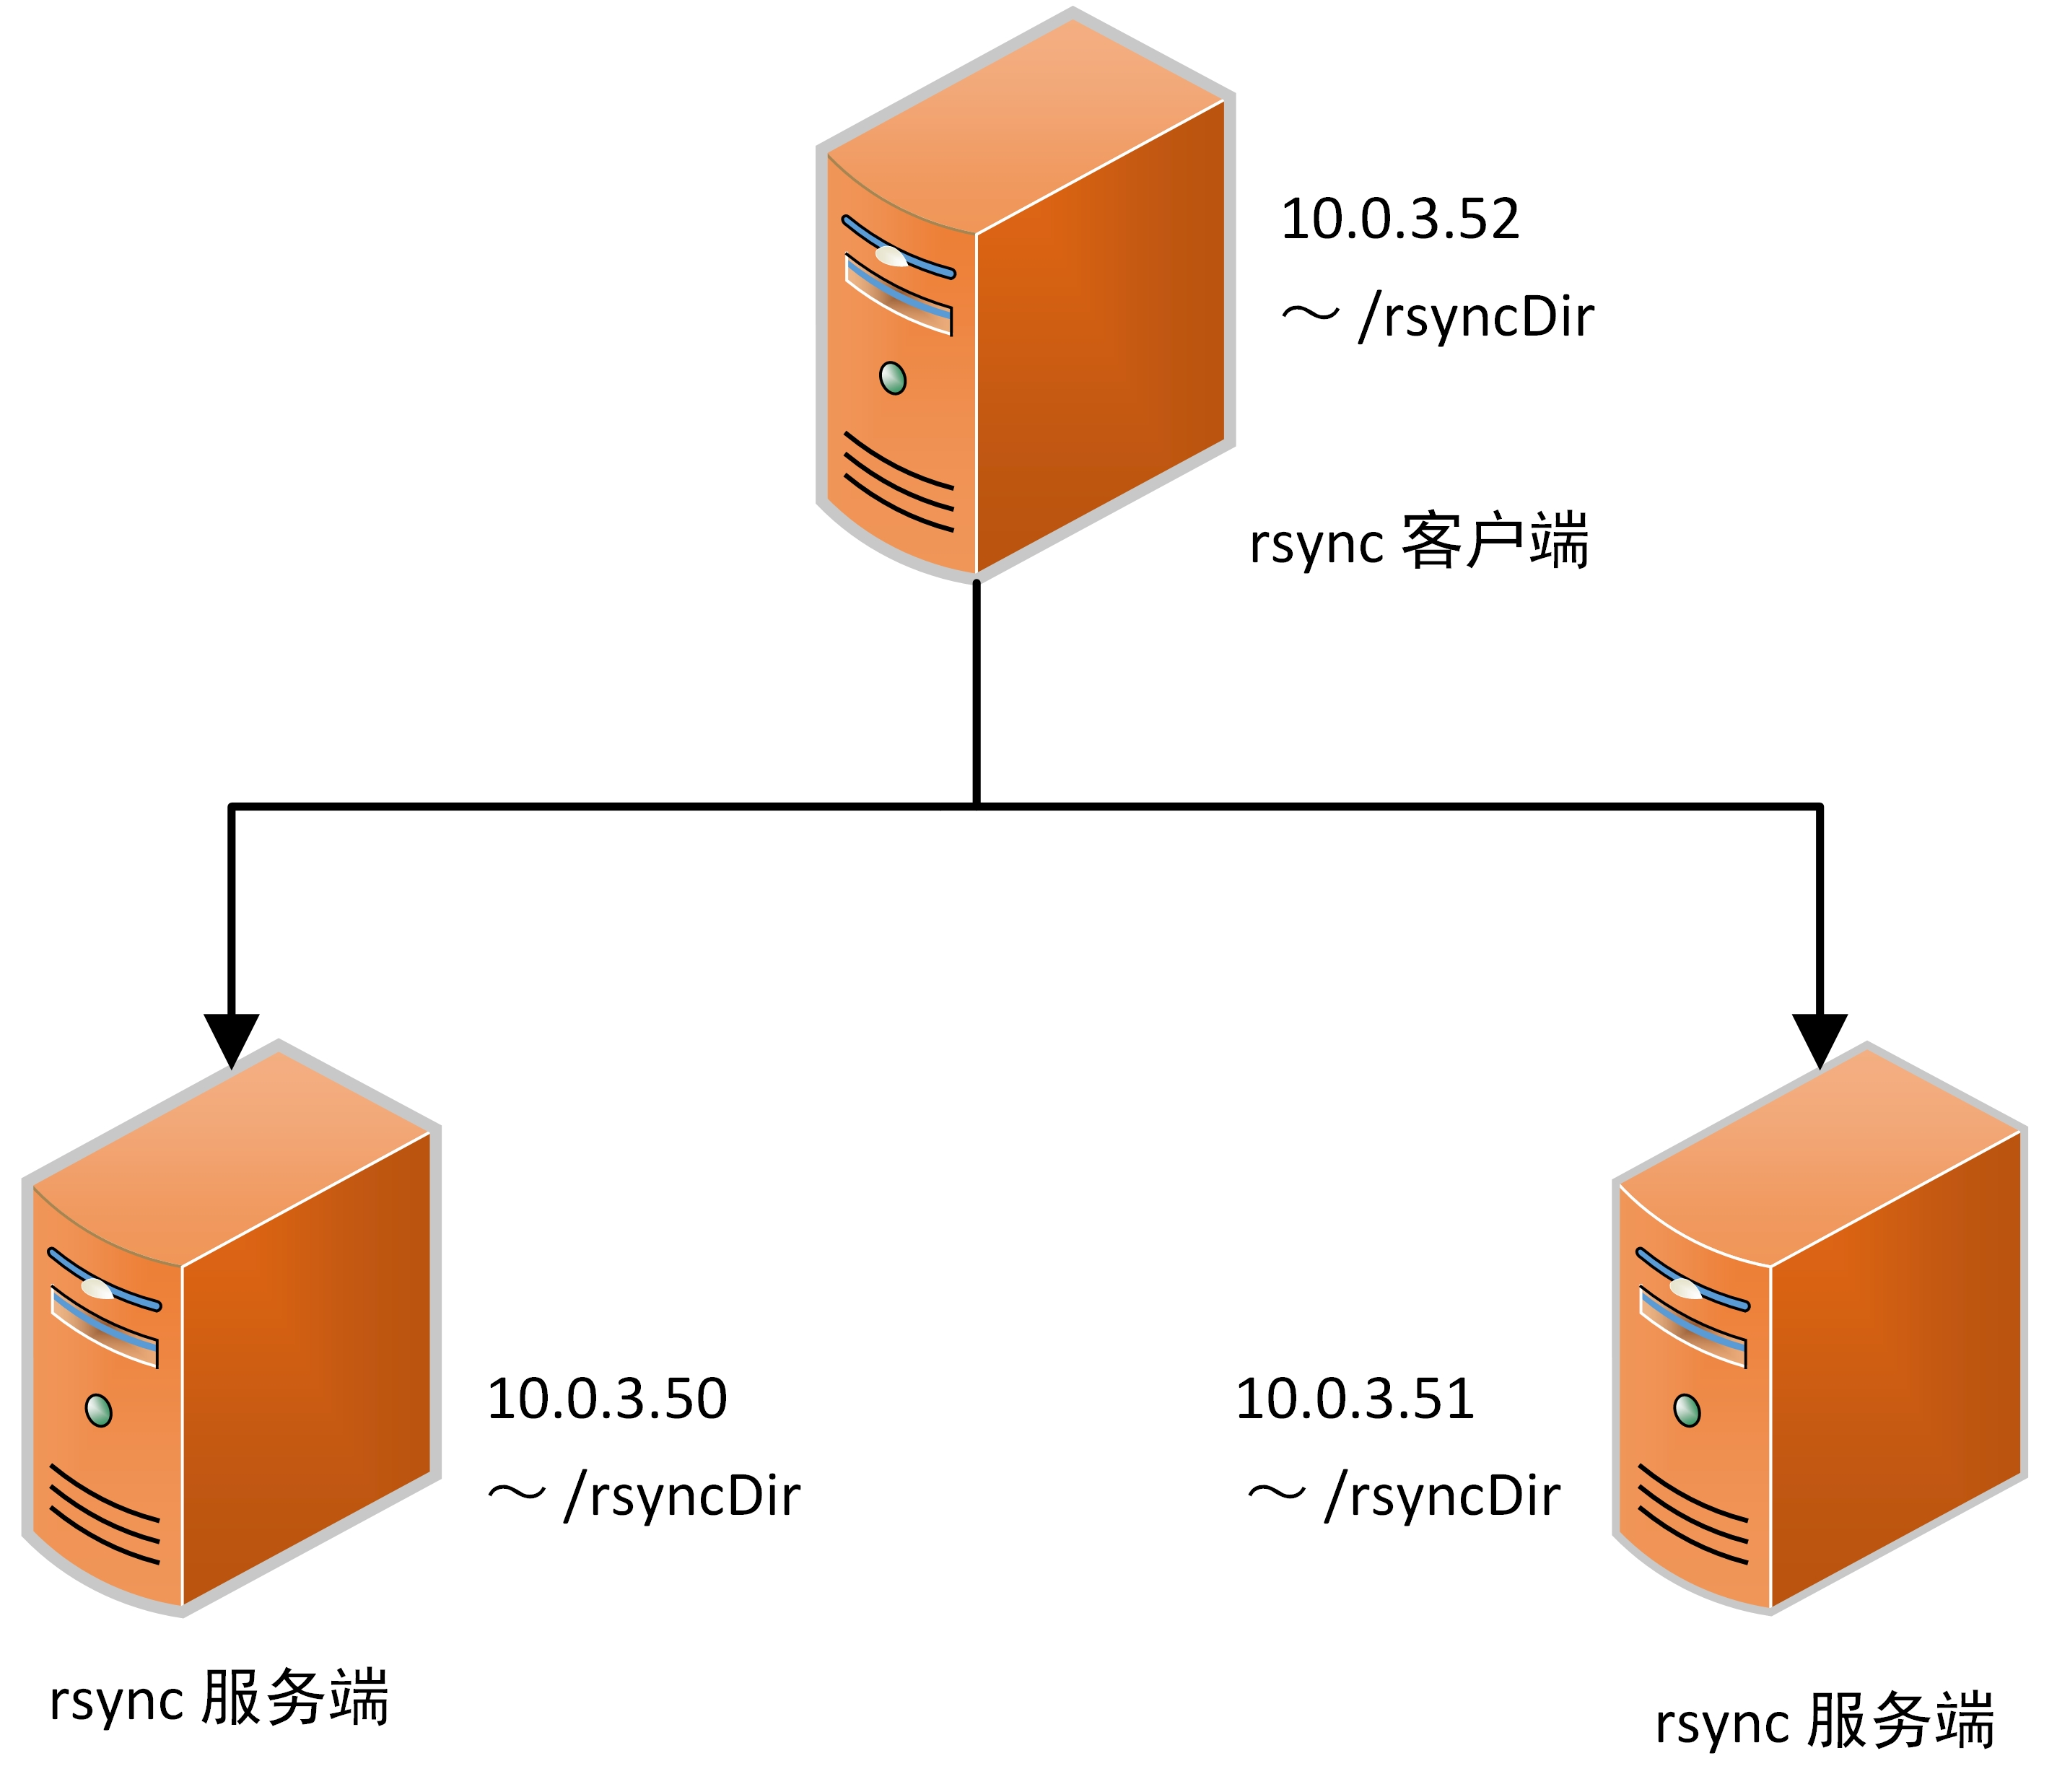
\includegraphics[width=\textwidth]{pic/rsync.jpg}
\caption{rsync}
\end{figure}
\subsection{安装}
服务端\footnote[1]{运行守护进程,故称之为服务端}两台机器上都安装如下包:\\
\shell{sudo apt-get install rsync -y}
\par
客户端安装如下包:\\
\shell{sudo apt-get install rsync inotify-tools -y}

\subsection{配置}
\subsubsection{服务端}
\shell{sudo mkdir /etc/rsyncd}\\
\shell{sudo vim /etc/rsyncd/rsyncd.conf}
添加如下内容:
\begin{verbatim}
uid = nobody
gid = nobody
use chroot = yes
max connections = 10
strict modes = yes              #检查口令文件
pid file = /var/run/rsyncd.pid
lock file = /var/run/rsync.lock
log file = /var/log/rsyncd.log

[rsyncUbuntu]
path = /home/ubuntu/rsyncDir    #同步路径
comment = rsyncUbuntu file
ignore errors                   #忽略无关的I/O错误
read only = no                  #可上传
write only = no                 #可下载
uid = ubuntu
gid = ubuntu
hosts allow = 10.0.3.0/24       #多个网段空格隔开
hosts deny = *
list = false                    #该模块不可列出
auth users = unisonA                    #认证用户名
secrets file = /etc/rsyncd/unisonA.pass #包含"用户名:密码"格式的文件
\end{verbatim}

另一台机器最后两行改为:\\
\texttt{auth users = unisonB}\\
\texttt{secrets file = /etc/rsyncd/unisonB.pass}

\par
分别创建密码文件:\\
\shell{sudo vim /etc/rsyncd/unisonA.pass}\\
\texttt{unisonA:ustc}\\
另一台机器做类似操作.

\par
该文件权限要求设置为进程所有者可读:\\
\shell{sudo chmod 600 /etc/rsyncd/unisonA.pass}\\
\shell{sudo chown root:root /etc/rsyncd/unisonA.pass}\\
另一台机器做类似操作.

\par
创建目标文件夹并运行守护进程:\\
\shell{mkdir $\sim$/rsyncDir}\\
\shell{sudo /usr/bin/rsync --daemon --config=/etc/rsyncd/rsyncd.conf}

\par
查看进程状态和监听端口:\\
\shell{ps -efA | grep rsync}\\
\shell{netstat -tunlp} \\
可以看到默认使用的端口为873.

\subsubsection{客户端}
\shell{sudo mkdir /etc/rsyncd}\\
\shell{sudo echo "ustc" /etc/rsyncd/unisonA.pass}\\
\shell{sudo echo "ustc" /etc/rsyncd/unisonB.pass}\\
\shell{sudo chmod 600 /etc/rsyncd/*.pass}\\
\shell{sudo chown ubuntu:ubuntu /etc/rsyncd/*.pass}\\
这里的密码文件同样要求只能为运行程序的所属者读取.

编写如下脚本:\\
\shell{vim $\sim$/rsync.sh}
\begin{verbatim}
#!/bin/bash
host1=10.0.3.50
host2=10.0.3.51
src=/home/ubuntu/rsyncDir/ #注意末尾是否加 / 的区别
dst1=rsyncUbuntu
dst2=rsyncUbuntu
user1=unisonA
user2=unisonB
/usr/bin/inotifywait -mrq --timefmt '%d/%m/%y %H:%M' --format '%T %w%f%e' \ 
-e close_write,modify,delete,create,attrib,move $src \
| while read files
    do
    /usr/bin/rsync -vzrtopg --delete \
        --progress --password-file=/etc/rsyncd/unisonA.pass \
        $src $user1@$host1::$dst1
    /usr/bin/rsync -vzrtopg --delete \
        --progress --password-file=/etc/rsyncd/unisonB.pass \
        $src $user2@$host2::$dst2
    done
\end{verbatim}

修改权限运行测试即可:\\
\shell{chmod +x rsync.sh}\\
\shell{./rsync.sh \&}\\
\shell{mkdir rsyncDir}

\par
我使用LXC完成的实验,遇到一个错误说找不到对应的模块``rsyncUbuntu",结果是服务端的允许网段设置错误,导致客户端连接被拒绝. 关于rsync.conf配置文件的更多信息见”有道笔记“或者官方文档. 